% !TeX spellcheck = cs_CZ
%{\tikzset{external/prefix={tikz/FYZI/}}
% \tikzset{external/figure name/.add={ch23_}{}}
%=========================== Kapitola: Rezonance ==================================================
\setchaptertoc
\chapter{Rezonance}\label{fyz:IchapXXIII}
  \section{Komplexní čísla a harmonický pohyb}\label{fyz:IchapXXIIIsecI}
    V této kapitole budeme pokračovat v diskuzi o harmonickém oscilátoru, zejména o harmonickém
    oscilátoru s nucenými kmity, přičemž v další analýze použijeme novou techniku. V předchozí
    kapitole jsme zavedli komplexní čísla s reálnou a imaginární částí, která lze znázomit graficky,
    přičemž na vodorovnou osu se vynáší reálná část a na svislou osu imaginární část. Komplexní
    číslo a můžeme zapsat jako \(a= a_r + \imath a_i\), kde index \(r\) znamená reálnou část \(a\) a
    index \(\imath\) znamená imaginární část \(a\). Víme, že komplexní číslo \(a = x + \imath y\)
    můžeme napsat i ve tvaru \(x + \imath y = r e^{\imath\vartheta}\), kde \(r^2 = x^2 + y^2 = (x +
    \imath y)(x - \imath y) = aa^*\) (obr. \ref{fyz:fig0415}). (Komplexně sdružené číslo \(a^*\) k
    číslu \(a\) dostaneme, když v \(a\) změníme znaménko u \(\imath\).) Komplexní číslo můžeme
    zapsat v libovolném z těchto dvou tvarů - udáním reálné a imaginární části nebo pomocí modulu
    \(r\) a fáze \(\vartheta\). Známe-li \(r\) a \(\vartheta\), jsou \(x\) a \(y\) rovny
    \(r\cos\vartheta\) a \(r\sin\vartheta\), nebo naopak, známe-li komplexní číslo ve tvaru \(x +
    \imath y\), je \(r= \sqrt{x^2 + y^2}\) a \(\tan\vartheta=\sfrac{y}{x}\) (tj. podíl imaginární a
    reálné části.)

    \begin{figure}[ht!] %\ref{fyz:fig0415}
      \centering
      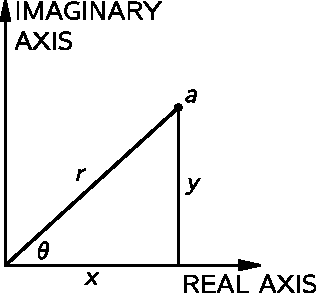
\includegraphics[width=0.3\linewidth]{fyz_fig0415.pdf}
      \caption{Komplexní číslo lze znázornit bodem v \uv{komplexní rovině}
               (\cite[s.~309]{Feynman01})}
      \label{fyz:fig0415}
    \end{figure}

    Použití komplexních čísel k analýze fyzikálních jevů nám umožní následující trik. Uváděli jsme
    příklady oscilátorů, buzených vnější silou, která je rovna - součinu konstanty \(F_0\) a
    \(\cos\omega \). Takovou sílu lze zapsat jako reálnou část komplexního čísla
    \(F_0\exp{\imath\omega t}\), neboť \(\exp{\imath\omega t} = \cos\omega t + \imath\sin\omega t\).
    Důvod, proč si ji zapíšeme v takovém tvaru, je ten, že s exponenciální funkcí se nám počítá
    snadněji než s kosinem. Celý trik tedy spočívá v tom, že naše oscilační funkce vyjádříme jako
    reálné části určitých komplexních funkcí. Takto definovaná komplexní veličina \(F\) není rovna
    skutečné fyzikální síle, neboť žádná fyzikální síla není komplexní. Skutečné síly nemají
    imaginární část, jen reálnou část. Dále však budeme \(F_0\exp{\imath\omega t}\) nazývat „silou“,
    i když je síla ve skutečnosti rovna reálné části tohoto výrazu.

    Uvedeme další příklad. Představme si, že takto chceme zapsat sílu s kosinovým průběhem a s
    fázovým zpožděním \(\Delta\). Bude to reálná část z \(F_0\exp{\imath(\omega t-\Delta)}\), ale
    exponenciály můžeme napsat jako \(\exp{\imath\omega t}\exp{-\imath\Delta}\). Vidíme, že s
    exponenciálními funkcemi se počítá podstatně snadněji než s funkcemi sinus a kosinus, a to je
    důvodem, proč jsme se rozhodli použít komplexní čísla. Často budeme psát
    \begin{equation}\label{fyz:eq989}
      F=F_0\exp{-\imath\Delta}\exp{\imath\omega t}=\hat{F}\exp{\imath\omega t}.
    \end{equation}
    Malá stříška nad \(F\) nám má připomínat, že jde o komplexní veličinu. V tomto případě
    \begin{equation*}
      \hat{F} = F_0\exp{-\imath\Delta}.
    \end{equation*}

    Použijme komplexní čísla k vyřešení nějaké rovnice, abychom se přesvědčili, zda jich lze využít
    v praktických situacích. Například zkusme vyřešit rovnici
    \begin{equation}\label{fyz:eq990}
      \diff[2]{x}{t}+\frac{kx}{m}=\frac{F}{m}=\frac{F_0}{m}\cos\omega t,
    \end{equation}
    kde \(F\) je budicí síla oscilátoru a \(x\) jeho výchylka. Ačkoli se to může zdát absurdní,
    předpokládejme čistě z matematického hlediska, že \(x\) a \(F\) jsou komplexní čísla, tj., že
    \(x\) má reálnou a imaginámí část, a podobně i \(F\). Rovnice \eqref{fyz:eq990} pak bude mít
    tvar
    \begin{align*}
      \diff[2]{(x_r+\imath x_i)}{t}+\frac{k(x_r+\imath x_i)}{m} 
        &= \frac{F_r+\imath F_i}{m}   \\
      \shortintertext{neboli}
      \diff[2]{x_r}{t}+\frac{kx_r}{m}+\imath\left(\diff[2]{x_i}{t}+\frac{kx_i}{m}\right) 
        &= \frac{F_r}{m}+\frac{\imath F_i}{m}.
    \end{align*}

    Protože dvě komplexní čísla jsou si rovna pouze tehdy, jsou-li si rovny jejich reálné a
    imaginární části, vyplývá z toho, že \emph{reálná část \(x\) splňuje rovnici s reálnou částí
    síly}. Musíme zdůraznit, že takové rozdělení na reálnou a imaginární část \emph{neplatí} obecně,
    ale jen pro \emph{lineární} rovnice, tj. rovnice, kde se \(x\) vyskytuje jen v první nebo nulté
    mocnině. Kdyby se tam například vyskytoval člen \(\lambda x^2\), pak bychom po dosazení \(x_r +
    \imath x_i\). dostali \(\lambda(x_r + \imath x_i)^2\) a po rozdělení na reálnou a imaginární
    část bychom dostali \(\lambda(x_r^2 - x_i^2)\) pro reálnou část a \(2\imath\lambda x_rx_i\) pro
    imaginámí část. V reálné části by se pak nenacházel jen člen \(\lambda x_r^2\), ale \(-\lambda
    x_i^2\). V takovém případě bychom dostali jinou rovnici, než je ta, kterou chceme řešit.
    Rovnici, v níž by bylo přimícháno i \(x_i\), veličina, kterou jsme do našich úvah zavedli úplně
    uměle.

    Zkusme podle naší nové metody najít řešení, které již známe. Jde o stejnou rovnici
    \eqref{fyz:eq990}, ale nyní ji zapíšeme jako
    \begin{equation}\label{fyz:eq991}
      \diff[2]{x}{t}+\frac{kx}{m}=\frac{\hat{F}\exp{\imath\omega t}}{m},
    \end{equation}

  \section{Tlumené nucené kmity}\label{fyz:IchapXXIIIsecII}

    \begin{figure}[ht!] %\ref{fyz:fig0416}
      \centering
      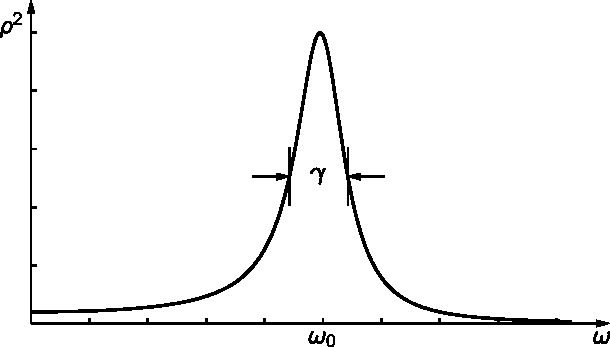
\includegraphics[width=0.7\linewidth]{fyz_fig0416.pdf}
      \caption{Graf \(\varrho^2\) v závislosti na \(\omega\)
              (\cite[s.~313]{Feynman01})}
      \label{fyz:fig0416}
    \end{figure}

    \begin{figure}[ht!] %\ref{fyz:fig0417}
      \centering
      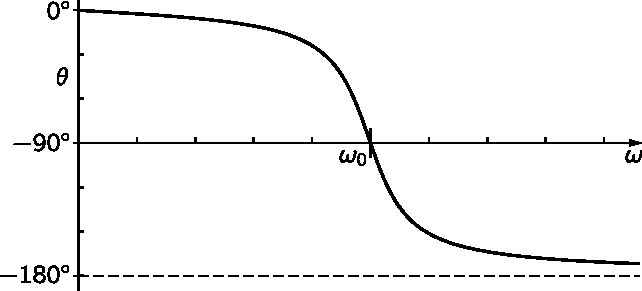
\includegraphics[width=0.7\linewidth]{fyz_fig0417.pdf}
      \caption{Graf \(\vartheta\) v závislosti na \(\omega\)
               (\cite[s.~314]{Feynman01})}
      \label{fyz:fig0417}
    \end{figure}

  \section{Rezonance v elektrických obvodech}\label{fyz:IchapXXIIIsecIII}

    \begin{figure}[ht!] %\ref{fyz:fig0418}
      \centering
      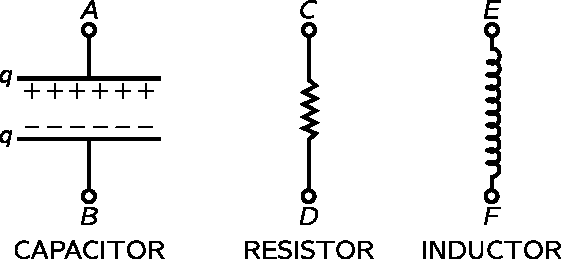
\includegraphics[width=0.5\linewidth]{fyz_fig0418.pdf}
      \caption{Tři pasivní prvky elektrických obvodů
              (\cite[s.~315]{Feynman01})}
      \label{fyz:fig0418}
    \end{figure}

    \begin{figure}[ht!] %\ref{fyz:fig0419}
      \centering
      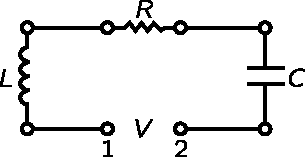
\includegraphics[width=0.3\linewidth]{fyz_fig0419.pdf}
      \caption{Elektrický oscilační obvod s odporem, cívkou a kondenzátorem
               (\cite[s.~316]{Feynman01})}
      \label{fyz:fig0419}
    \end{figure}

  \section{Rezonance v přírodě}\label{fyz:IchapXXIIIsecIV}

    \begin{figure}[ht!] %\ref{fyz:fig0420}
      \centering
      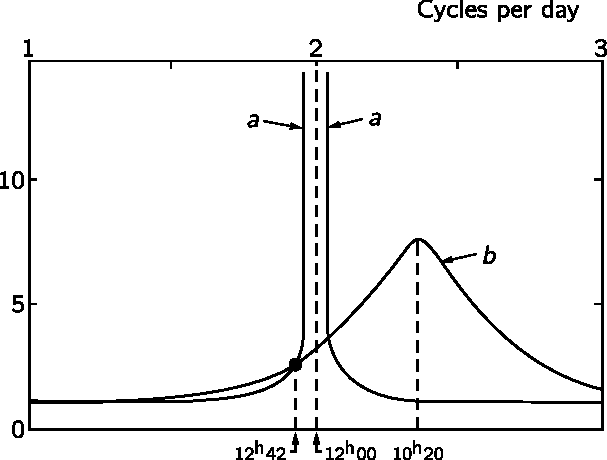
\includegraphics[width=0.7\linewidth]{fyz_fig0420.pdf}
      \caption{Reakce atmosféry na vnější excitace. Křivka \(a\) zobrazuje očekávanou reakci na
              atmosférický příliv a odliv typu \(S_2\) způsobený gravitací Měsíce: zvětšení v maximu
              je \(100:1\). Křivka \(b\) představuje průběh odvozený z pozorovaného zvětšení a fáze
              přílivu a odlivu typu \(M_2\). (\cite[s.~318]{Feynman01})}
      \label{fyz:fig0420}
    \end{figure}

    \begin{figure}[ht!] %\ref{fyz:fig0421}
      \centering
      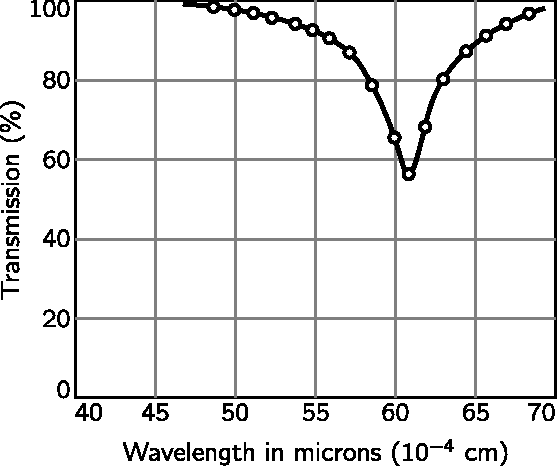
\includegraphics[width=0.7\linewidth]{fyz_fig0421.pdf}
      \caption{Koeficient průchodu infračerveného záření tenkou
               (\protect\SI{0.17}{\protect\micro\protect\m}) vrstvou chloridu sodného
               (\cite[s.~319]{Feynman01})}
      \label{fyz:fig0421}
    \end{figure}
  
    \begin{figure}[ht!] %\ref{fyz:fig0422}
      \centering
      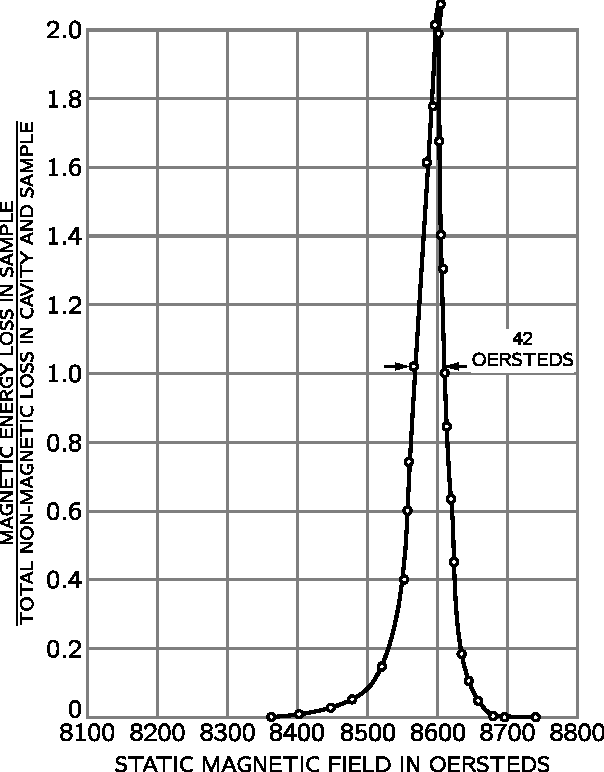
\includegraphics[width=0.7\linewidth]{fyz_fig0422.pdf}
      \caption{Ztráta energie v paramagnetické organické sloučenině v závislosti na intenzitě
               vnějšího magnetického pole (1 oersted = \protect\SI{1/4\pi
               e3}{\protect\ampere\protect\per\protect\meter}) (\cite[s.~320]{Feynman01})}
      \label{fyz:fig0422}
    \end{figure}
  
    \begin{figure}[ht!] %\ref{fyz:fig0423}
      \centering
      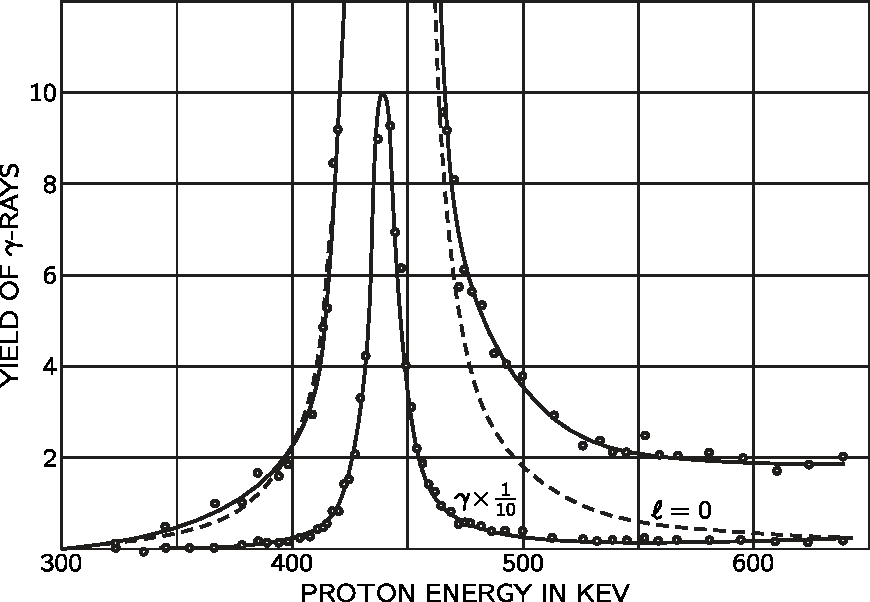
\includegraphics[width=0.7\linewidth]{fyz_fig0423.pdf}
      \caption{Intenzita gama záření lithia jako funkce energie bombardující protonů. Přerušovaná 
               čára představuje teoretický výpočet pro protony s momentem hybnosti \(l=0\)
               (\cite[s.~320]{Feynman01})}
      \label{fyz:fig0423}
    \end{figure}
  
    \begin{figure}[ht!] %\ref{fyz:fig0424}
      \centering
      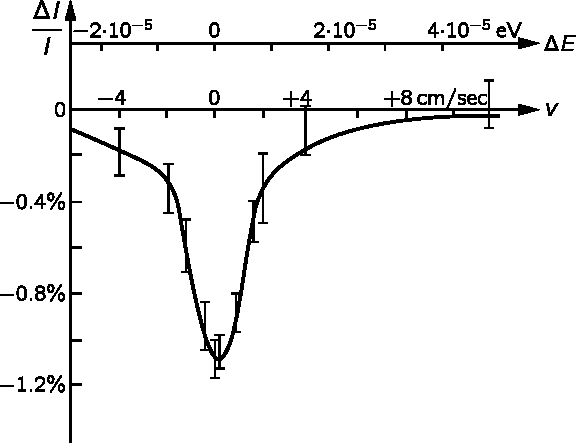
\includegraphics[width=0.7\linewidth]{fyz_fig0424.pdf}
      \caption{S laskavostí Dr. R. M\"{o}ssbauera
               (\cite[s.~321]{Feynman01})}
      \label{fyz:fig0424}
    \end{figure}
  
    \begin{figure}[ht!] %\ref{fyz:fig0425}
      \centering
      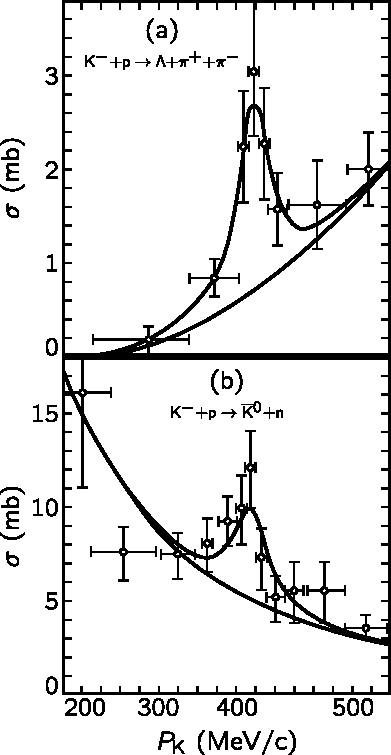
\includegraphics[width=0.6\linewidth]{fyz_fig0425.pdf}
      \caption{Závislost účinného průřezu na hybnosti reakce: a) \(K^+ + p \rightarrow \Lambda + \pi
              + \pi^-\) b) \(K^- + p \rightarrow K^o + n\); Dolní křivky \(a\) i \(b\) představují
              předpokládané pozadí bez rezonance, zatímco horní křivky obsahují ještě navíc
              superponovanou rezonanci; srážkový průřez je v 1 mb =
              \protect\SI{e-25}{\protect\m\protect\squared} (\cite[s.~321]{Feynman01})}
      \label{fyz:fig0425}
    \end{figure}

  \section{Příklady a cvičení}\label{fyz:IchapXXIIIsecV}
%---------------------------------------------------------------------------------------------------